\documentclass[12pt]{article}
\usepackage[serbian]{babel}
\usepackage[T2A]{fontenc}
\usepackage[utf8]{inputenc}
\usepackage{amssymb,amsthm,amsmath}
\usepackage{amsfonts}
\usepackage{yhmath}
\usepackage{lipsum}
\usepackage{graphicx}
\usepackage[margin=2.2cm]{geometry}
\usepackage{listings}
\usepackage{xcolor}
\usepackage{tocloft}
\usepackage{helvet}
\usepackage{listings}
\usepackage{tocbibind}
\usepackage{array,booktabs}
\usepackage{multirow}
\usepackage{amsmath}
\theoremstyle{definition}
\newtheorem{definition}{Definicija}[section]
\theoremstyle{remark}
\newtheorem*{remark}{Primer}
\usepackage{hyperref}
\pagestyle{plain}



\hypersetup{
    colorlinks=true,
    linkcolor=black,
    citecolor=black,
    urlcolor=blue, 
    linktoc=all,
    linkbordercolor=white,
    urlbordercolor=white,
    citebordercolor=white
}

\definecolor{codegreen}{rgb}{0,0.6,0}
\definecolor{codegray}{rgb}{0.5,0.5,0.5}
\definecolor{codepurple}{rgb}{0.58,0,0.82}
\definecolor{backcolour}{rgb}{0.95,0.95,0.92}

\lstdefinestyle{mystyle}{
    backgroundcolor=\color{backcolour},   
    commentstyle=\color{codegreen},
    keywordstyle=\color{magenta},
    numberstyle=\tiny\color{codegray},
    stringstyle=\color{codepurple},
    basicstyle=\ttfamily\footnotesize,
    breakatwhitespace=false,         
    breaklines=true,                 
    captionpos=b,                    
    keepspaces=true,                 
    numbers=left,                    
    numbersep=5pt,                  
    showspaces=false,                
    showstringspaces=false,
    showtabs=false,                  
    tabsize=2
}

\lstset{style=mystyle}

\pagestyle{empty}
\begin{document}

\begin{titlepage}
\noindent\begin{minipage}{0.5\linewidth}
\Large Matematički fakultet,\newline
Univerzitet u Beogradu
\end{minipage}
\vspace{7cm}

\noindent\hrulefill
\begin{center}
    {\it\large Fakultetski projekat}
    
    \vspace{0.25cm}
    {\bf\LARGE Predviđanje bankrota kompanija }
\end{center}
\hrulefill

\vspace{8cm}

\noindent\begin{minipage}{0.5\linewidth}
\Large\sc Staša Tonić 157/2019\newline
Natalija Lazić 230/2018 \newline
Оgnjen Đuković 8/2018
\end{minipage}

\vfill
\begin{center}
    \Large Maj 2023.
\end{center}
\end{titlepage}
\renewcommand\contentsname{Sadržaj}
\tableofcontents\thispagestyle{empty}\newpage

\section{Uvod}
\vspace{0.5 cm}
Globalna ekonomska kriza $2008.$ godine pokrenula je mnoge razgovore na temu stabilnosti tržišta i poslovanja kompanija, kao i alata koji se mogu upotrebiti da se isti predvide. 

Modeli koji mogu predvideti bankrot od velike su važnosti ne samo za pojedinačne kompanije, već i za globalnu ekonomiju. Oni mogu pomoći investitorima i drugim zainteresovanim stranama da procene finansijski rizik pri ulaganju u određenu kompaniju, analitičarima da uoče kompanije koje su u finansijskoj opasnosti, samim kompanijama da uoče probleme u svom poslovanju i na vreme preduzmu potrebne mere za prevenciju bankrota, poput smanjenja troškova, promene načina poslovanja, povećanja prihoda i slično. Korišćenje ovih modela takođe može pomoći pri donošenju bolje informisanih odluka kada su u pitanju kupovina i prodaja akcija, izbor dobavljača ili kupaca, kao i odobravanje kredita. Ideja iza njih je posmatranje i analiziranje KPI-jeva (Key Performance Indictors) koji predstavljaju metrike koje kompanije koriste kako bi procenile svoj uspeh u ispunjavanju određenih poslovnih ciljeva i objektiva. Neki od čestih KPI-jeva za procenu finansijski performansi su profitabilnost, rast prihoda i odnos duga i kapitala. Njihova analiza može ukazati na određene poteškoće u poslovanju i predvideti da li kompanija pokazuje simptome bankrotstva ili ne. Uočavanje poteškoća nadalje pomaže kompaniji da donese odgovarajuće odluke.  

Kada kompanija bankrotira, postoje dva moguća scenarija - može pokušati reorganizaciju putem unapred pripremljenog plana reorganizacije (UPPR) ili otići pod stečaj, što znači da se automutoski povlači sa Beogradske berze. Stečaj može biti prijavljen od strane same kompanije ili nekog od njenih poverioca. Odlazak pod stečaj podrazumeva da je poslovni model te kompanije došao u situaciju gde više nije održiv i nije u stanju da izmiri svoje dugove. Kompanija se likvidira i sud postavlja stečajnog upravnika koji pokreće formalni proces u okviru kog se imovina te kompanije prodaje da bi se namirili njeni poverioci. Nadalje se resursi kompanije raspoređuju u između poverioca u skladu sa zakonom. Prodaja imovine može se odnositi na prodaju zaliha, opreme, nekretnina i drugih imovinskih predmeta. Nakon što su svi dugovi isplaćeni, preostala sredstva se distribuiraju vlasnicima kompanije ili drugim povezanim stranama i tada se likvidacija kompanije završava. Međutim, može se desiti da sredstva od prodaje imovine nisu dovoljna da se izmire sve finansijske obaveze. Ukoliko se to desi, poverioci će biti izmireni prema prioritizaciji koju propisuje zakon - uobičajeno je da se prvo izmire dugovi prema poveriocima koji imaju obezbeđenje na imovini kompanije (npr. hipoteku), zatim se izmiruju porezi i doprinosi, a na kraju se izmiruju neplaćeni dugovi. Ukoliko prihod od prodaje imovine ne pokrije sva dugovanja, preostali dugovi će ostati neizmireni. Odlazak pod stečaj predstavlja veoma  komplikovan i dug proces koji može trajati nekoliko meseci ili, u zavisnosti od veličine i složenosti kompanije, čak i godina.

\newpage 

\section{Opis baze i priprema podataka za obradu}
\vspace{0.5 cm}

Baza podataka koju ćemo koristiti za analizu sastoji se od podataka prikupljenih iz  \emph{Taiwan Economic Journal}-a za godine $1999$ - $2009$. Bankrot kompanije definisan je na osnovu poslovnih propisa tajvanske berze. 

Skup podataka se sastoji od zavisne promenljive koja nosi informaciju o tome da li je kompanija bankrotirala i $95$ prediktora. Zavisna promenljiva je binarnog tipa, gde $1$ predstavlja bankrot, dok $0$ označava da je kompanija nastavila da postoji. Prediktori obuhvataju različite informacije o poslovanju kompanije poput povraćaja sredstava, bruto dobiti, operativnih i neto prihoda i rashoda, tokova novca, dugovanja itd. Baza se sastoji od $6819$ opservacija.

Baza podataka ima stroge zahteve za kompanije uključene u njenu analizu. Prvo, sve kompanije moraju imati na raspolaganju najmanje tri godine potpunih javnih informacija pre nego što dožive finansijsku krizu. Pored toga, zbog potreba poređenja, skup podataka uključuje samo kompanije sa značajnim brojem sličnih kompanija u industriji.

Skup podataka čine proizvodne kompanije, sa $346$ firmi u industrijskom i elektronskom sektoru, te $39$ uslužnih preduzeća i $93$ kompanije iz drugih sektora. Zbog neravnomerne raspodele kompanija u ovim kategorijama, podaci su veoma nebalansirani, što predstavlja izazov za tačna predviđanja prilikom primene našeg modela na širu populaciju kompanija.

Svi podaci unutar baze  su potpuni i skalirani između $0$ i $1$  korišćenjem formule: 
\begingroup
\large
$$x_{skalirano}=\frac{x-x_{min}}{x_{max}-x_{min}}$$
\endgroup

U okviru projekta predstavićemo različite algoritme klasifikacije na skupu podataka u cilju predviđanja bankrota kompanija sa zadovoljavajućom tačnošću mnogo pre stvarnog događaja.
Valja napomenuti da je za ovakvu vrstu problema, pored tačnosti predviđanja, neizostavan faktor i isplativost. Kao što se može zaključiti, mnogo je isplativije predvideti da će kompanija bankrotirati i da ta pretpostavka ne bude tačna, nego obrnuto.  

\subsection{Grafički prikaz podataka} 

%FALI HEAD, TJ. prikaz baze

Skup podataka sadrži tri kategoričke promenljive, pri čemu je kategorička promenljiva \emph{Net Income Flag}, koja predstavlja oznaku neto prihoda, za sve kompanije jednaka $1$.  Ovo ukazuje da je neto prihod za poslednje dve godine bio negativan u okviru svake kompanije, te je možemo isključiti iz dalje analize.

Kategorička promenljiva \emph{Liability-Assets Flag} daje informaciju o tome da li ukupna obaveza premašuje ukupnu imovinu, tj. da li kompanija duguje više novca od vrednosti onoga što poseduje. Ova pojava zabeležena je samo kod $6$ kompanija.

Na sledećem \emph{bar plot}-u možemo videti broj kompanija koje su bankrotirale i broj kompanija koje nisu. Primećujemo da je broj kompanija koje nisu bankrotirale znatno veći od onih koje su doživele bankrot.

    \noindent\begin{minipage}{0.5\linewidth}
    \centering
    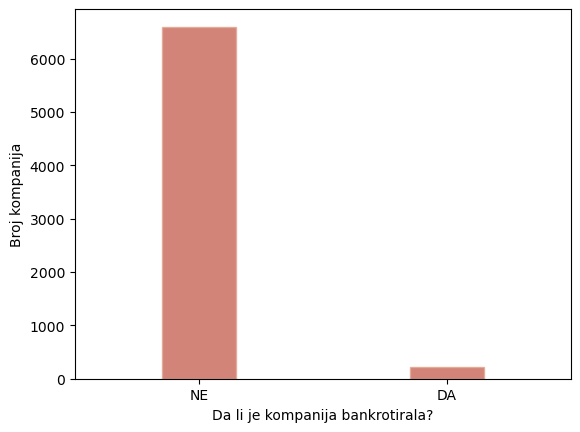
\includegraphics[width=0.95\linewidth]{barplot1.png}\newline
    \phantom{aaaa}
\end{minipage}
\begin{minipage}{0.5\linewidth}
    \centering
    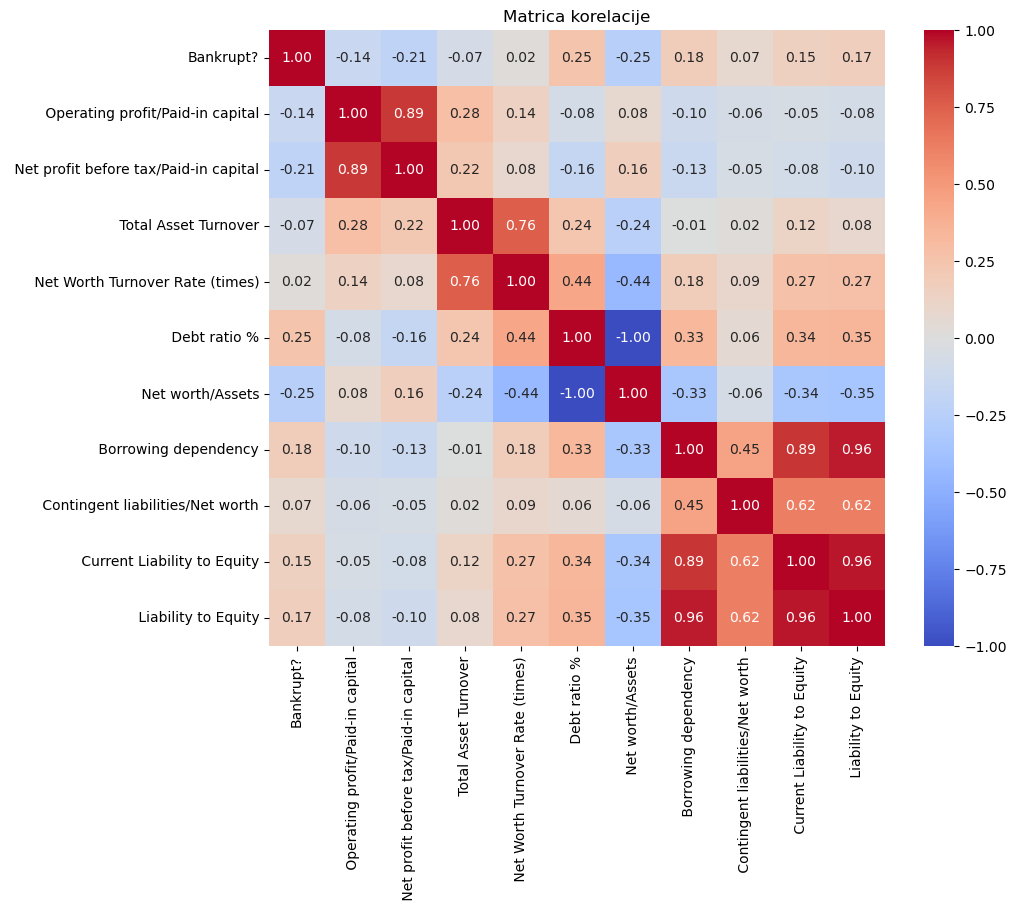
\includegraphics[width=1\linewidth]{slika2.png}\newline
    \phantom{aaaa}
\end{minipage}

Linearnu zavisnost varijabli možemo prikazati pomoću matrice korelacije. Na slikama su izdvojene značajne veze između prediktora kao i njihova korelisanost sa zavisnom promenljivom.

Primećujemo da su varijable \emph{Operating profit/Paid-in capital} i \emph{ Net profit before tax/Paid-in capital} pozitivno korelisane, kao i  \emph{Borrowing dependency}, \emph{Contingent liabilities/Net worth}, \emph{Current Liability to Equity} i \emph{Liability to Equity}.

Promenljive \emph{Debt ratio \%} i \emph{Net worth/Assets} su negativno korelisane, sa visokom stopom korelacije.

Takođe, promećujemo da su promenljive  \emph{ Net Value Per Share (B)},  \emph{Net Value Per Share (A)} i  \emph{ Net Value Per Share (C)} visoko pozitivno korelisane. 

Analogno primećujemo veze i između ostalih prediktora. Valja napomenuti da korelacija pojedinačnih prediktora sa zavisnom promenljivom postoji, ali se ne može smatrati  statistički značajnom. 
\vspace{0.4cm}

\noindent\begin{minipage}{0.5\linewidth}
    \centering
    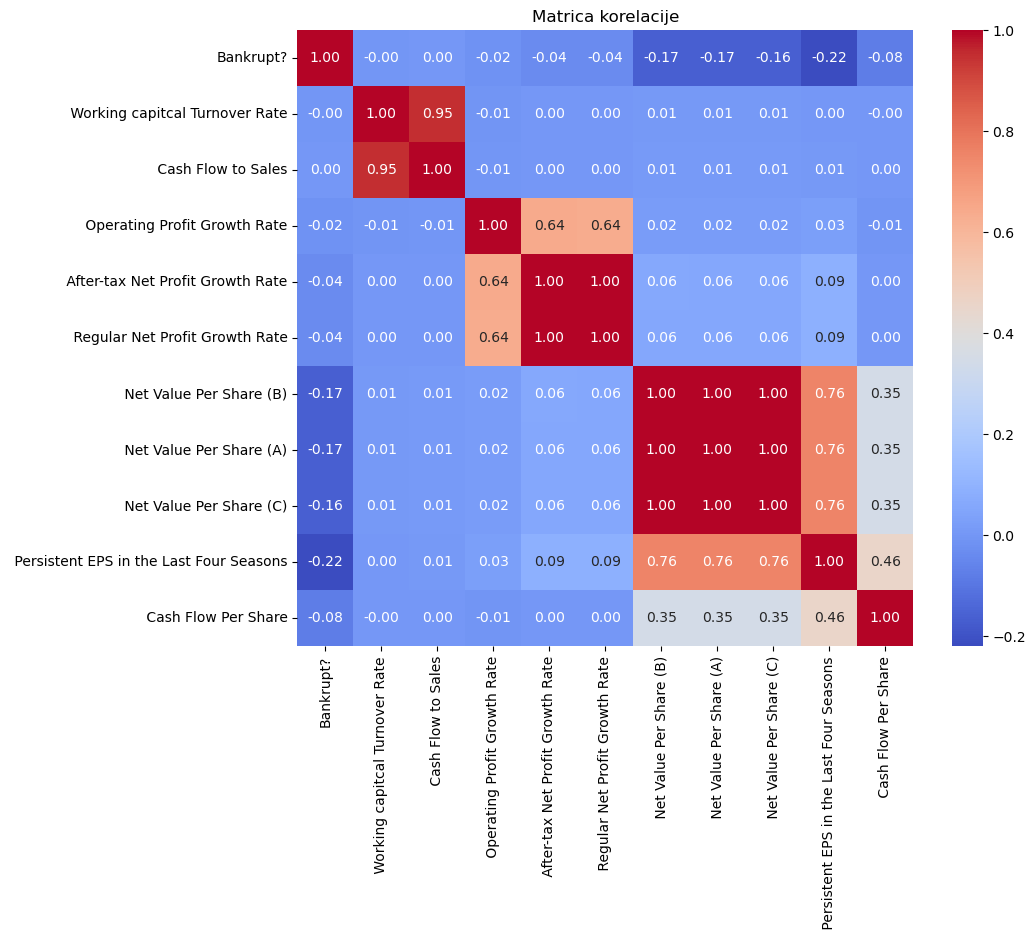
\includegraphics[width=1\linewidth]{slika1.png}\newline
    
\end{minipage}
\begin{minipage}{0.5\linewidth}
    \centering
    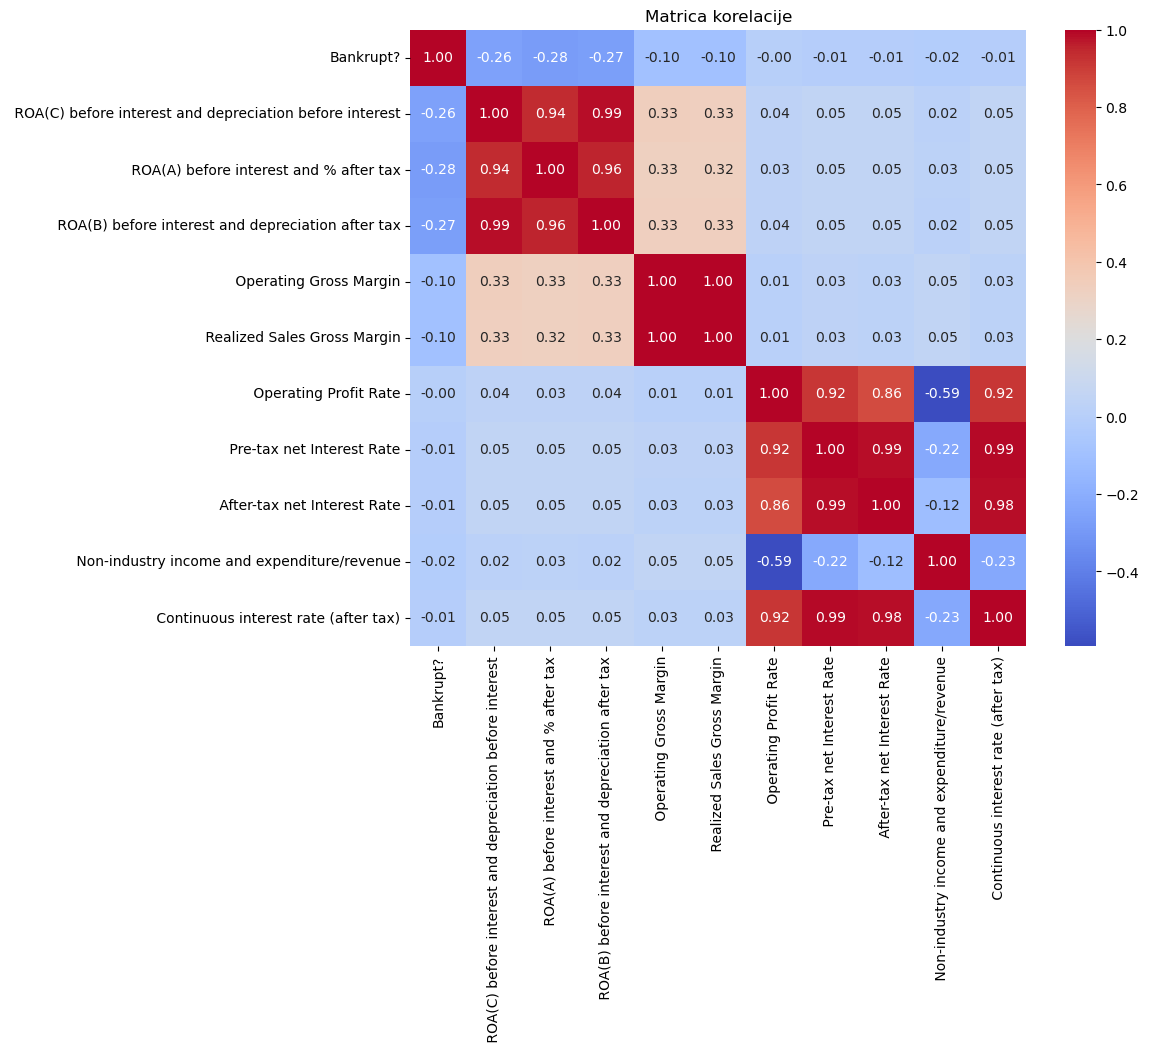
\includegraphics[width=1\linewidth]{slika3.png}\newline
     
\end{minipage}




\newpage

\subsection{Metode balansiranja podataka} 

Neuravnoteženost u bazi podataka odnosi se na situaciju kada postoje značajne razlike u broju primeraka različitih klasa u skupu podataka. U ovom slučaju, klasa kompanija koje su banrkotirale ima znatno manje primeraka od klase kompanija koje nisu bankrotirale, što može imati ozbiljne posledice za analizu podataka i performanse modela mašinskog učenja. Zbog ove devijacije, modeli će se više fokusirati na učenje kako klasifikovati veću klasu. 

Gorepomenuti problem možemo demostrirati na primeru modela
\emph{$k$ najbližih suseda (kNN)}. Očekujemo da će ovaj model predvideti da skoro nijedna kompanija neće bankrotirati. 

Pre konsturisanja modela, potrebno je podeliti podatke na test i trening skupove:

\hfill
\lstinputlisting[language=Python, firstline=71, lastline=73]
{kod.py}

\hfill

Kao što smo već pomenuli, podaci unutar baze su unapred skalirani. Sada možemo primeniti \emph{kNN} algoritam za proizvoljno $k$, npr. $k=10$ i konstruisati naš model na sledeći način:

\hfill
\lstinputlisting[language=Python, firstline=75, lastline=77]
{kod.py}

\hfill



Grafički prikaz matrice konfuzije daje nam uvid u broj ispravno i pogrešno klasificiranih instanci za svaku klasu.

\begin{figure}[htp]
    \centering
    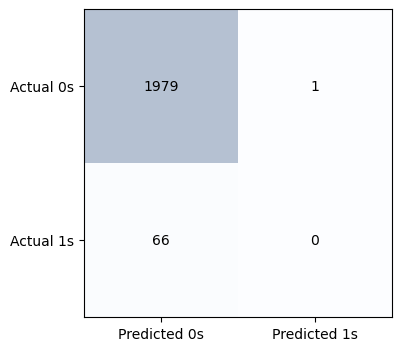
\includegraphics[width=6.5cm]{output_6_0.png}
    \caption{Matrica konfuzije}
    \label{fig:galaxy}
\end{figure}

%Rekla mi je drugrica sa ETFa da bas mnog koriste te termine ova greska nas vise kosta skuplja je itd da je to taj sleng pa sam toupotrebila
Matrica konfuzije ovog modela nam govori da naš klasifikator nije dobar jer pravi veliki broj $skupljih$ grešaka. Dakle, mnogo je veći broj kompanija koje su bankrotirale, premda je naš model predvideo da će njihov način poslovanja biti održiv, nego obrnuto. Kao što smo već napomenuli, ovaj tip grešaka je puno manje isplativ od predviđanja bankrota unutar kompanija koje će nastaviti da postoje.


Postoje različite strategije koje se mogu primeniti za rešavanje problema neuravnoteženosti podataka. Neke od mogućih strategija su:
\renewcommand\labelitemi{\tiny$\bullet$}
\begin{itemize}

    \item \emph{Biranje dobre funkcije evaluacije} - U slučaju neuravnotežene baze podataka, model koji pretežno predviđa dominantnu klasu može imati visoku vrednost funkcije   \emph{accuracy}, iako je prilično neuspešan prilikom predviđanja manje zastupljenih klasa. Stoga, prilikom rada sa neuravnoteženim podacima, za funkciju evaluacije treba odabrati neku od funkcija \emph{Precision}, \emph{Recall}, \emph{F1 Score} i slično.
    \item \emph{Reuzorkovanje (Resampling)} - Metodološki pristup koji se koristi za rešavanje problema neuravnoteženih podataka tako što manipuliše veličinom uzorka podataka u cilju poboljšanja performansi modela mašinskog učenja. Osnovni tipovi reuzorkovanja su \emph{undersampling} (podselekcija) i \emph{oversampling} (prekomerna selekcija). 
\end{itemize}



\subsubsection{Undersampling}

Podselekcija, tj.\emph{undersampling} je tehnika koja podrazumeva smanjenje broja uzoraka zastupljenije klase u cilju ravnoteže između klasa. Na primer, neka klasu $1$ čini $1000$ uzoraka, a klasu $2$ čini $100$ uzoraka. Prilikom korišćenja ove metode, iz klase $1$ uzimamo $100$ uzoraka, te je nakon primene \emph{undersampling}-a broj uzoraka u obe klase izbalansiran.

Potrebno je napomenuti da ova tehnika može dovesti do preterane prilagođenosti, tj. \emph{overfitting}-a modela, kao i gubitka informacija iz podataka. Zbog svega navedenog, \emph{undersampling} se koristi samo u slučaju kada je to neophodno i kada se očekuje da broj uzoraka neće uticati na performanse modela.

U nastavku ćemo pokazati primenu \emph{undersampling}-a na realnim podacima. Koristićemo ovu tehniku da rešimo problem neuravnoteženih podataka, te napraviti model korišćenjem \emph{kNN} algoritma na sređenim podacima.


Pre konstrukcije modela, potrebno je da ranije definisane trening skupove podelimo tako što ćemo razdvojiti kompanije unutar njih na osnovu toga da li su bankrotirale ili ne. Segregaciju vršimo na sledeći način:

\hfill
\lstinputlisting[language=Python, firstline=81, lastline=84]
{kod.py}

\hfill

Pravimo novi trening skup koji će se sastojati iz izbalansiranih (uravnoteženih) podataka:

\hfill
\lstinputlisting[language=Python, firstline=85, lastline=92]
{kod.py}

\hfill

  Sada možemo primeniti \emph{kNN} algoritam. Uzećemo da je $k=15$, kao vrednost broja $k$ za koju smo dobili najbolje predviđanje. Konstruišemo naš model i njegovu matricu konfuzije kao:

\hfill
\lstinputlisting[language=Python, firstline=94, lastline=96]
{kod.py}

\hfill

Matrica konfuzije novog modela ukazuje na primetno bolje performanse istog, što možemo zaključiti na osnovu njenog grafičkog prikaza:

 \begin{figure}[htp]
    \centering
    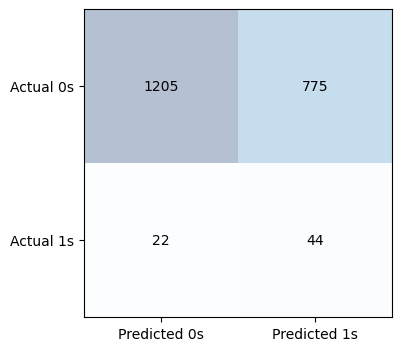
\includegraphics[width=7cm]{output_12_0.png}
    \caption{Matrica konfuzije za \emph{undersampling} model}
    \label{fig:galaxy}
\end{figure}

Primećujemo da se broj grešaka prve vrste smanjio, što možemo navesti kao primaran cilj ove popravke modela. Takođe, možemo videti da se broj grešaka druge vrste, takozvanih \emph{lažnih uzbuna}, znatno povećao. Međutim, kao što smo ranije napomenuli, veći broj grešaka druge vrste je i dalje isplativiji u kontekstu predikcije ishoda o budućnosti kompanija.  

Kao mere kvaliteta u cilju procene performansi našeg modela koristimo funkcije evaluacije  \emph{F1 Score}, \emph{AUC ROC} i \emph{Precision}. Njihovom primenom dobijamo sledeće rezultate:

\hfill
\lstinputlisting[language=Python, firstline=99, lastline=99]{kod.py}
$$
\text{F1 Score : 0.43}
$$
$$
\text{AUC ROC : 0.63}
$$
$$
\text{Precision : 0.05}
$$
\hfill


\emph{F1 Score} od $0.43$ govori da naš model ima određeni nivo efikasnosti prilikom identifikacije pozitivnih instanci dok minimizira lažno pozitivne i lažno negativne instance.

 Vrednost \emph{AUC ROC}-a je $0.64$, što implicira da model ima umerenu diskriminatornu moć u razlikovanju pozitivnih i negativnih instanci. Ova vrednost sugeriše da model funkcioniše bolje od slučajnog nagađanja, ali da nije veoma precizan u svojim predviđanjima.

Preciznost modela od $0.05$ ukazuje na to da model ima veoma nisku sposobnost da ispravno identifikuje pozitivne instance. Dakle, od svih slučajeva koje je model predvideo kao pozitivne, samo $5\%$ njih je stvarno pozitivno, dok je preostalih $95\%$ lažno pozitivno.\\



 %PROKOMENTARISALA, PROVERI DA LI JE DOBRO

 U slučaju kada ne želimo da se odreknemo podataka, možemo napraviti više uravnoteženih trening skupova. Sastojaće se od kompanija koje su bankrotirale, dok će kompanije koje nisu bankrotirale biti jednako raspodeljene svakom od njih. 
 
 Za početak, određujemo broj trening skupova koje ćemo koristiti za pravljenje modela:
\vspace{0.1cm} 
\hfill
\lstinputlisting[language=Python, firstline=101, lastline=101]
{kod.py}
\hfill


Ukupan broj trening skupova biće $29$. Konstruišemo ih kao:

\hfill
\lstinputlisting[language=Python, firstline=103, lastline=116]
{kod.py}

\hfill


Ovom implementacijom odrekli smo se podataka o određenom broju kompanija koji je jednak ostatku pri deljenju $\frac{N}{n}$. Kako taj broj ne može biti previše veliki, izbacivanje kompanija iz modela ne bi trebalo značajno uticati na isti.


Sada možemo primeniti \emph{kNN} algoritam za $k=15$ na svaki od novonastalih trening skupova:


\hfill
\lstinputlisting[language=Python, firstline=118, lastline=130]
{kod.py}

\hfill

Kao konačnu procenu uzećemo ocenu koja se najčešće pojavljuje u svim modelima:

\hfill
\lstinputlisting[language=Python, firstline=132, lastline=132]
{kod.py}

\hfill

Konstruišemo matricu konfuzije modela koji čini $29$ trening skupova i grafički je prikazujemo:

\begin{figure}[htp]
    \centering
    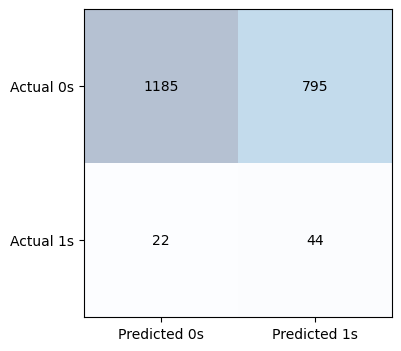
\includegraphics[width=7cm]{output_20_0.png}
    \caption{Matrica konfuzije za \emph{undersampling} model}
    \label{fig:galaxy}
\end{figure}

Kao mere kvaliteta u cilju procene performansi našeg novog modela koristimo funkcije evaluacije  \emph{F1 Score}, \emph{AUC ROC} i \emph{Precision}. Njihovom primenom dobijamo sledeće rezultate:

\hfill
\lstinputlisting[language=Python, firstline=135, lastline=135]{kod.py}
$$
\text{F1 Score : 0.42}
$$
$$
\text{AUC ROC : 0.63}
$$
$$
\text{Precision : 0.05}
$$
\hfill

Možemo primetiti da ove vrednosti funkcija evaluacije nisu bolji od rezultata dovijenih na osnovu modela koji čini jedan trening skup. Međutim, od velikog su značaja zato što, usled ovako definisane implementacije, znamo da njihove vrednosti nisu posledica \emph{overfitting}-a.


Ukoliko smatramo da je svaki podatak neizostavan, možemo, na primer, gorepomenuti ostatak kompanija podeliti po trening skupovima. Oni će tada imati jednu kompaniju koja nije bankrotirala više od ostalih, što neće negativno uticati na model. Međutim, primenom ovog postupka ne očekujemo bitno drugačije rezultate u odnosu na prethodnu diskusiju.

\subsubsection{Oversampling}

Prekomerna selekcija, tj. \emph{oversampling} je tehnika koja podrazumeva dodavanje novih uzoraka u manje zastupljenu klasu u cilju ravnoteže između klasa. Ova tehnika se najčešće primenjuje kada je broj uzoraka bitan faktor u performansama modela.

Najjednostavniji pristup u okviru \emph{oversampling}-a je umnožavanje postojećih uzoraka manje zastupljene klase, što se naziva \emph{up-sampling}. Na primer, neka klasu $1$ čini $1000$ uzoraka, a klasu $2$ čini $100$ uzoraka. Prilikom korišćenja ove metode možemo udesetostručiti broj uzoraka klase $2$ i time izbalansirati broj uzoraka u obe klase. 

Potrebno je napomenuti da ova tehnika može dovesti do preterane prilagođenosti, tj. \emph{overfitting}-a modela, kao i gubitka informacija iz podataka. Do gubitka informacija dolazi jer se postojeći uzorci ponavljaju bez dodavanja novih informacija. Zbog svega navedenog, često se primenjuju složenije tehnike \emph{oversampling}-a, kao što su SMOTE (\emph{Synthetic Minority Over-sampling Technique}) i ADASYN (\emph{Adaptive Synthetic Sampling}) tehnike.

U nastavku ćemo pokazati primenu SMOTE tehnike na realnim podacima. Koristićemo ovu tehniku da rešimo problem neuravnoteženih podataka, te napraviti model korišćenjem \emph{kNN} algoritma na sređenim podacima. 


\hfill
\lstinputlisting[language=Python, firstline=138, lastline=139]
{kod.py}

\hfill

Sada možemo primeniti \emph{kNN} algoritam. Ovako definisan trening skup sastoji od velikog broja elemenata, te je potrebno da broj $k$ bude dovoljno veliki.  Uzećemo da je $k=150$, kao vrednost broja $k$ za koju smo dobili dobre rezultate. Konstruišemo naš model i matricu konfuzije kao:

\hfill
\lstinputlisting[language=Python, firstline=141, lastline=144]
{kod.py}

\hfill

Grafički prikazujemo matricu konfuzije našeg modela:

\begin{figure}[htp]
    \centering
    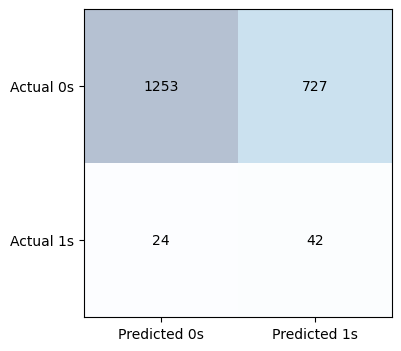
\includegraphics[width=7cm]{output_27_0.png}
    \caption{Matrica konfuzije za \emph{oversampling} model}
    \label{fig:galaxy}
\end{figure}

Kao i do sad, kao mere kvaliteta koristimo funkcije evaluacije \emph{F1 Score}, \emph{AUC ROC} i \emph{Precision}. Njihovom primenom dobijamo sledeće rezultate:

\hfill
\lstinputlisting[language=Python, firstline=147, lastline=147]{kod.py}
$$
\text{F1 Score : 0.44}
$$
$$
\text{AUC ROC : 0.63}
$$
$$
\text{Precision : 0.05}
$$
\hfill

Možemo primetiti da matrica konfuzije ovog modela ne daje primetno bolje rezultate. Takođe, vrednosti funkcija evaluacije su zanemarljivo različite u odnosu na \emph{undersampling} tehniku. 

Dakle, možemo zaključiti da obe metode balansiranja podataka, prilikom obrade podatka iz zadate baze, imaju određeni nivo efikasnosti i u nekoj meri poboljšavaju model. Ipak, na osnovu rezultata primećujemo da predikcije koje naš model pravi i nakon ove korekcije nisu najpouzdanije.

\newpage
\subsection{Metode redukcije dimenzionalnosti podataka}

Baza podataka koju analiziramo sastoji se od velikog broja prediktora. U okviru grafičke analize podataka, primetili smo da su mnogi od njih su međusobno korelisani. Pojava korelacije među prediktorima može dovesti do problema prilikom analize, interpretacije i vizualizacije podataka. 

Kako bismo rešili problem korelacije između prediktora, možemo koristiti neku od sledećih metoda:

\begin{itemize}

\item \emph{Odabir prediktora (Feature Selection)} - Pristup koji za konstrukciju modela bira najrelevantnije prediktore i izostavlja one koji su visoko međusobno korelisani. Neke od tehnika koje se mogu koristiti za implementaciju ove metode su \emph{ANOVA}, \emph {Ridge} i \emph {Lasso} regresija.

\item \emph{ Smanjenje broja prediktora (Feature Extraction)} - Pristup koji koristi matematičke tehnike za transformisanje originalnih prediktora u novi, kompaktniji skup prediktora. Novonastali skup će imati manju dimenziju i zadržaće što više informacija koje je inicijalni skup prediktora posedovao. Neki od algoritama za smanjenje broja prediktora su \emph{Principal Component Analysis (PCA)}, \emph{t-distributed Stochastic Neighbor Embedding (t-SNE)} i  \emph{Uniform Manifold Approximation and Projection for Dimension Reduction (UMAP)}.

\item  \emph{ Metode ansambla (Ensemble Methods)} - Pristup koji podrazumeva kombinaciju različitih algoritama za smanjenje dimenzionalnosti podataka.


\end{itemize}


\subsubsection{PCA - Analiza glavnih komponenti}

Pokazaćemo primenu \emph{Analize glavnih komponenti} na realnim podacima. Koristićemo ovu tehniku da smanjimo dimenzionalnost i rešimo problem korelacije između prediktora, te napraviti model logističke regresije na osnovu sređenih podataka.


Kao i ranije, podatke unutar baze delimo na test i trening skup. Zatim pravimo transformaciju našeg trening skupa u okviru koje njegovi prediktori postaju glavne komponente:

\hfill
\lstinputlisting[language=Python, firstline=149, lastline=152]
{kod.py}

\hfill

Nacrtaćemo grafik kumulativne sume disperzije, te na osnovu njega pokušati da zaključimo koliko infomacija prilikom redukcije zadržava svaka dimenzija i identifikujemo one dimenzije koje doprinose većoj varijabilnosti. 

\begin{figure}[htp]
    \centering
    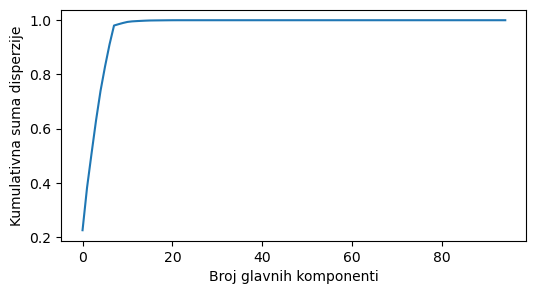
\includegraphics[width=10cm]{output_31_0.png}
    \caption{Grafik kumulativne sume disperzije}
    \label{fig:galaxy}
\end{figure}

\newpage

Cilj nam je da pronađemo dovoljan broj glavnih komponenti, tako da njihov udeo u disperziji bude $99\%$. To možemo uraditi na sledeći način:

\hfill
\lstinputlisting[language=Python, firstline=154, lastline=155]
{kod.py}

\hfill

Dakle, dovoljan broj glavnih komponenti čije disperzije čine $99\%$ ukupne disperzije je $11$. Nacrtaćemo sada grafik udela u disperziji svake od glavnih komponenata.

\begin{figure}[htp]
    \centering
    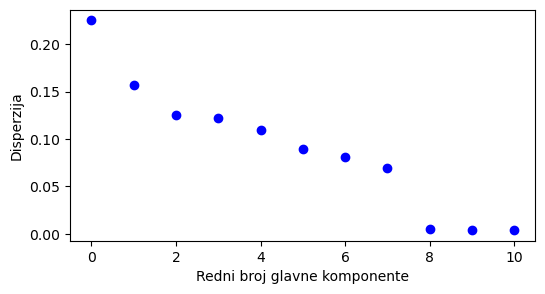
\includegraphics[width=10cm]{output_33_0.png}
    \caption{Grafik udela svake glavne komponente u disperziji}
    \label{fig:galaxy}
\end{figure}

Na ovaj način konstruisali smo matricu transformacije dimenzije $95\times 11$. Nju ćemo iskorisiti za transformaciju našeg trening i test skupa, te na novodobijeni trening skup primeniti logističku regresiju kao:


\hfill

\lstinputlisting[language=Python, firstline=159, lastline=163]
{kod.py}

\hfill


Rezultati dobijeni konstrukcijom ovog modela bitno se ne razlikuju od prethodno navedenih, što možemo videti na osnovu grafičkog prikaza matrice konfuzije:

\begin{figure}[htp]
    \centering
    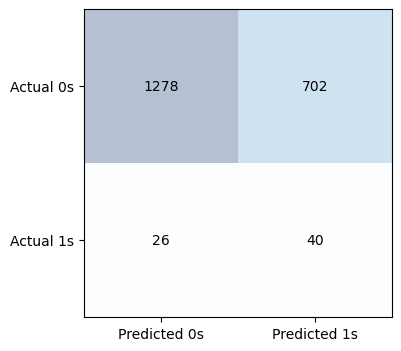
\includegraphics[width=7cm]{output_35_0.png}
    \caption{Matrica konfuzije za logističku regresiju}
    \label{fig:galaxy}
\end{figure}

Kao i do sad, kao mere kvaliteta u cilju procene performansi modela logističke regresije koristimo funkcije evaluacije  \emph{F1 Score}, \emph{AUC ROC} i \emph{Precision}. Njihovom primenom dobijamo sledeće rezultate:

\hfill
\lstinputlisting[language=Python, firstline=166, lastline=166]{kod.py}
$$
\text{F1 Score : 0.44}
$$
$$
\text{AUC ROC : 0.63}
$$
$$
\text{Precision : 0.05}
$$
\hfill

Kako se rezultati dobijeni modelom logističke regresije značajno ne razlikuju od prethodno dobijenih vrednosti, možemo analogno izvesti zaključke o kvalitetu modela.\\


Valja napomenuti i da možemo kombinovati \emph{Analizu glavnih komponenti} PCA i prethodno navedenu tehniku \emph{oversampling}-a pod nazivom SMOTE. Ovim postupkom dobijamo uravnoteženu bazu na kojoj možemo primeniti \emph{kNN} algoritam. 

Demonstriraćemo opisani postupak na podacima iz naše baze podataka korišćenjem sledećih funkcija:

\hfill
\lstinputlisting[language=Python, firstline=168, lastline=171]{kod.py}

Kao i do sada, tačnost modela dobijenog kombinovanjem ove dve metode i \emph{kNN} algoritma proveravamo preko matrice konfuzije. Posmatrajmo njen grafički prikaz:
 
\begin{figure}[htp]
    \centering
    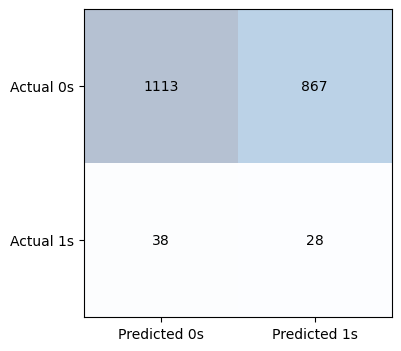
\includegraphics[width=7cm]{output_39_0.png}
    \caption{Matrica konfuzije za PCA i SMOTE tehniku}
    \label{fig:galaxy}
\end{figure}

\newpage

Kao i do sad, kao mere kvaliteta u cilju procene performansi našeg modela koristimo funkcije evaluacije  \emph{F1 Score}, \emph{AUC ROC} i \emph{Precision}. Njihovom primenom dobijamo sledeće rezultate:

\hfill
\lstinputlisting[language=Python, firstline=174, lastline=174]{kod.py}
$$
\text{F1 Score : 0.38}
$$
$$
\text{AUC ROC : 0.49}
$$
$$
\text{Precision : 0.03}
$$
\hfill

Možemo primetiti rezultati funkcija evaluacije modela dobijenog korišćenjem \emph{Analize glavnih komponenti} PCA i SMOTE tehnike u kombinaciji sa \emph{kNN} algoritmom za nijansu gori od rezultata ostalih modela koje smo koristili.

\subsubsection{UMAP - Uniformna aproksimacija i projekcija prostora}

Uniformna aproksimacija i projekcija prostora, tj. \emph{Uniform Manifold Approximation and Projection} UMAP je algoritam koji se koristi za redukciju dimenzionalnosti, vizualizaciju i analizu visokodimenzionih podataka. 

Najčešće za novu dimenziju podataka uzimaju se brojevi $2$ ili $3$ kako bi se podaci mogli grafički predstaviti. Ovim algoritmom prvo smanjujemo dimenziju cele baze, a zatim konstruišemo trening i test skup. 

Glavna mana UMAP-a leži u tome što nemamo mogućnost direktnog ubacivanja novih podataka u model, već je prilikom dodavanja novih podataka potrebno ispočetka ponoviti konstrukciju modela.


Primenićemo UMAP algoritam na realne podatke iz naše baze. Za početak ćemo svesti bazu na dve dimenzije, pa podeliti podatke na trening i test skupove na sledeći način:

\hfill
\lstinputlisting[language=Python, firstline=176, lastline=178]{kod.py}

\hfill

Kako je dimenzija nove baze $2$, podatke možemo vizuelno prikazati u dvodimenzionalnom sistemu pomoću sledećeg grafika:


\begin{figure}[htp]
    \centering
    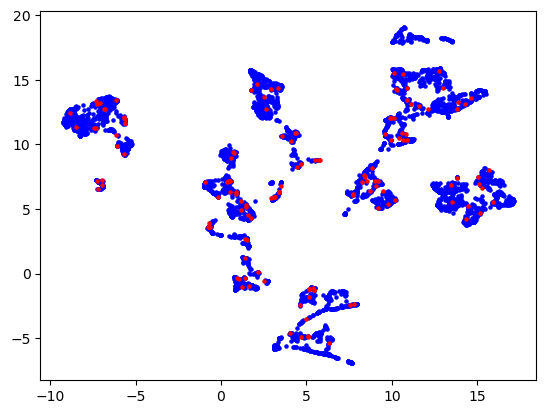
\includegraphics[width=0.45\textwidth]{output_43_0.png}
    \caption{Grafik podataka korišćenjem UMAP algoritma}
    \label{fig:galaxy}
\end{figure}

Pošto na grafiku ne uočavamo jasnu razdvojenost podataka, možemo proširiti trening skup koristeći gorepomenutu \emph{oversampling}-a pod nazivom SMOTE:

\hfill
\lstinputlisting[language=Python, firstline=181, lastline=182]{kod.py}

\hfill

Nakon primene ove tehnike, ponavljamo postupak grafičkog prikazivanja dobijenih podataka i tada dobijamo:



\begin{figure}[htp]
    \centering
    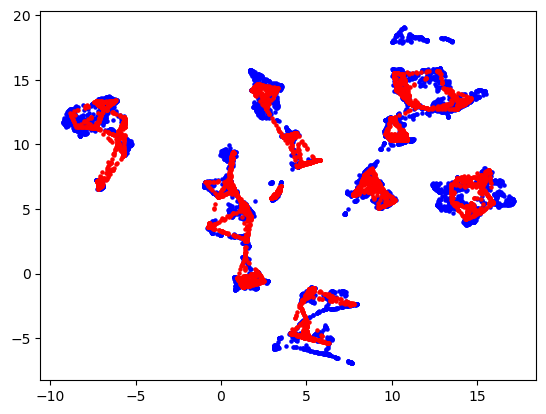
\includegraphics[width=0.45\textwidth]{output_46_0.png}
    \caption{Grafik podataka korišćenjem UMAP algoritma i SMOTE tehnike}
    \label{fig:galaxy}
\end{figure}

Vidimo da i dalje ne postoji jasna razdvojenost između kompanija, ali možemo primetiti da na određenim mestima postoje mali klasteri tačaka iste boje. Ova pojava nam implicira da možemo isprobati \emph{kNN} algoritam. Kako klasteri koje smo uočili nisu veliki, za vrednost broja $k$ uzećemo $k=50$ i primeniti algoritam:

\hfill
\lstinputlisting[language=Python, firstline=184, lastline=186]
{kod.py}

\hfill

Za određivanje preciznosti modela ponovo koristimo matricu konfuzije. Posmatrajmo njen grafički prikaz:

\begin{figure}[htp]
    \centering
    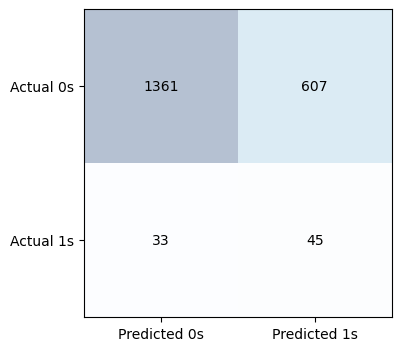
\includegraphics[width=8cm]{output_48_0.png}
    \caption{Matrica konfuzije za UMAP i SMOTE tehniku}
    \label{fig:galaxy}
\end{figure}

Kao i do sad, kao mere kvaliteta u cilju procene performansi našeg modela koristimo funkcije evaluacije  \emph{F1 Score}, \emph{AUC ROC} i \emph{Precision}. Njihovom primenom dobijamo sledeće rezultate:

\hfill
\lstinputlisting[language=Python, firstline=189, lastline=189]
{kod.py}
$$
\text{F1 Score : 0.47}
$$
$$
\text{AUC ROC : 0.63}
$$
$$
\text{Precision : 0.07}
$$

\hfill

Rezultati koje smo dobili slični su rezultatima dobijenim korišćenjem običnog trening skupa. Ovaj ishod je očekivan, jer je ideja UMAP algoritma da se prilikom preslikavanja tačaka u manjedimenzioni prostor čuvaju odnosi između njihovi rastojanja. Naime, cilj algoritma je da tačke koje su se nalazile blizu u početnom prostoru budu blisko pozicionirane u prostoru nove dimenzije i obratno. \\

Ponovo ćemo primeniti UMAP algoritam na realne podatke iz naše baze. Sada ćemo svesti bazu na tri dimenzije, pa podeliti podatke na trening i test skupove na sledeći način:


\hfill
\lstinputlisting[language=Python, firstline=191, lastline=194]
{kod.py}

\hfill

Kako je dimenzija nove baze $3$, podatke možemo prikazati u trodimenzionalnom sistemu pomoću sledećeg grafika:

\begin{figure}[htp]
    \centering
    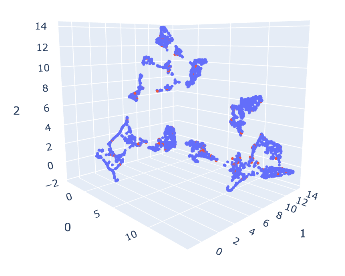
\includegraphics[width=7.5cm]{prvi3dgrafik.png}
    \caption{Grafik podataka korišćenjem UMAP algoritma}
    \label{fig:galaxy}
\end{figure}

Kao i malopre, na grafiku ne uočavamo jasnu razdvojenost podatka, te proširujemo trening skup koristeći SMOTE tehniku:


\hfill
\lstinputlisting[language=Python, firstline=197, lastline=199]
{kod.py}

\hfill

Nakon primene ove tehnike, ponavljamo postupak grafičkog prikazivanja dobijenih podataka i tada dobijamo:

\begin{figure}[htp]
    \centering
    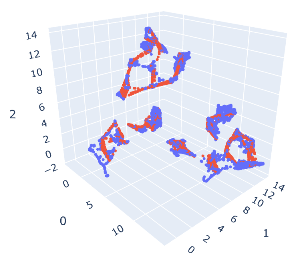
\includegraphics[width=7.5cm]{drugi3dgrafik.png}
    \caption{Grafik podataka korišćenjem UMAP algoritma i SMOTE tehnike}
    \label{fig:galaxy}
\end{figure}
\newpage

Vidimo da i dalje ne postoji jasna razdvojenost između kompanija, ali možemo primetiti da na određenim mestima postoje mali klasteri tačaka iste boje. Ponavljamo postupak odozgo i na novodobijene podatke primenjujemo \emph{kNN} algoritam. Kako klasteri koje smo uočili nisu veliki, za vrednost broja $k$ uzećemo $k=50$ i primeniti algoritam:

\hfill
\lstinputlisting[language=Python, firstline=201, lastline=203]
{kod.py}

\hfill

Za određivanje preciznosti modela ponovo koristimo matricu konfuzije i njen grafički prikaz:

\begin{figure}[htp]
    \centering
    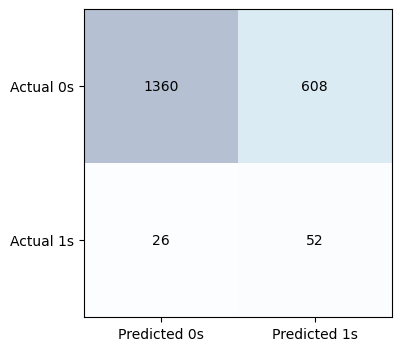
\includegraphics[width=8cm]{output_55_0.png}
    \caption{Matrica konfuzije za UMAP i SMOTE tehniku}
    \label{fig:galaxy}
\end{figure}

Kao i do sad, kao mere kvaliteta u cilju procene performansi našeg modela koristimo funkcije evaluacije  \emph{F1 Score}, \emph{AUC ROC} i \emph{Precision}. Njihovom primenom dobijamo sledeće rezultate:

\hfill
\lstinputlisting[language=Python, firstline=206, lastline=206]
{kod.py}
$$
\text{F1 Score : 0.48}
$$
$$
\text{AUC ROC : 0.68}
$$
$$
\text{Precision : 0.08}
$$ 

\hfill

Primećujemo da su rezultati koje smo dobili za ovaj model za nijansu bolji od rezultata modela čija baza ima dimenziju $2$, što je bilo i očekivano.\\

Valja napomenuti da se na skoro identičan način kao UMAP primenjuje i t-SNE algoritam, koji ovom prilikom nećemo detaljnije obraditi.


\subsubsection{Kombinacija PCA-a i UMAP-a}

Kao što smo već istakli, prilikom obrade podataka možemo kombinovati i različite metode smanjivanja dimenzije. Na realnim podacima iz naše baze upotrebićemo PCA, a zatim UMAP, te posmatrati podatke dobijene kombinacijom ovih metoda.

Treba istaći da ovaj pristup može biti koristan jer PCA smanjuje dimenzionalnost podataka, a UMAP dodatno smanjuje dimenzionalnost i čuva lokalne strukture podataka. 

Za početak, upotrebljavamo PCA i UMAP, te delimo dobijene podatke na test i trening skupove na sledeći način:

\hfill
\lstinputlisting[language=Python, firstline=208, lastline=212]
{kod.py}

\hfill


Kako je dimenzija nove baze $2$, podatke dobijene korišćenjem ove dve metode možemo prikazati u dvodimenzionalnom sistemu pomoću sledećeg grafika:

\begin{figure}[htp]
    \centering
    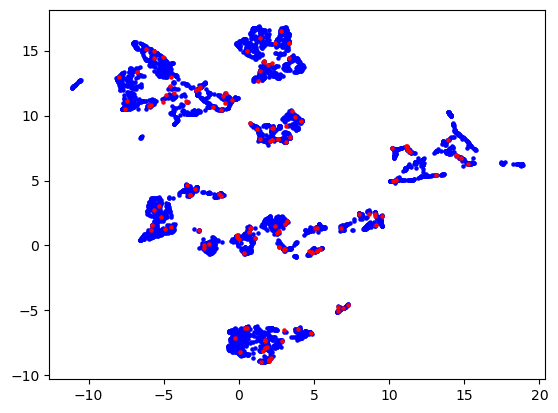
\includegraphics[width=7.5cm]{output_60_0.png}
    \caption{Grafik podataka korišćenjem PCA i UMAP algoritma}
    \label{fig:galaxy}
\end{figure}

Ponovo na grafiku ne uočavamo jasnu rasdvojenost podataka, te proširujemo trening skup koristeći SMOTE tehniku:

\hfill
\lstinputlisting[language=Python, firstline=214, lastline=215]
{kod.py}

\hfill
\newpage
Nakon primene ove tehnike, ponavljamo postupak grafičkog prikazivanja dobijenih podataka i dobijamo:

\begin{figure}[htp]
    \centering
    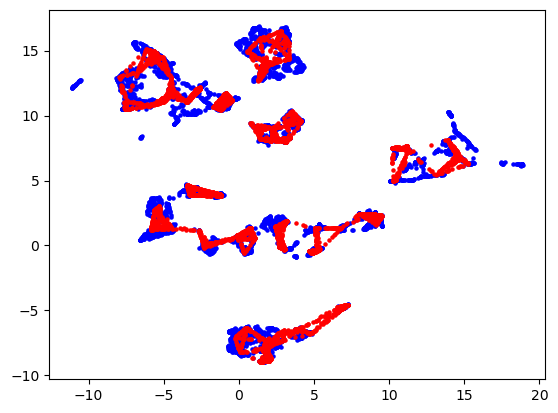
\includegraphics[width=7.5cm]{output_61_0.png}
    \caption{Grafik podataka korišćenjem PCA, UMAP i SMOTE tehnike}
    \label{fig:galaxy}
\end{figure}

Vidimo da i dalje ne postoji jasna razdvojenost između kompanija, ali možemo primetiti da na određenim mestima postoje mali klasteri tačaka iste boje. Ponavljamo postupak odozgo i na novodobijene podatke primenjujemo \emph{kNN} algoritam. Kako klasteri koje smo uočili nisu veliki, za vrednost broja $k$ uzećemo $k=50$ i primeniti algoritam:

\hfill
\lstinputlisting[language=Python, firstline=217, lastline=219]
{kod.py}

\hfill

Za određivanje preciznosti modela ponovo koristimo matricu konfuzije i njen grafički prikaz:

\begin{figure}[htp]
    \centering
    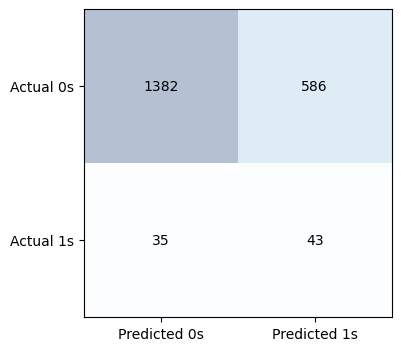
\includegraphics[width=8cm]{output_62_0.png}
    \caption{Matrica konfuzije za PCA, UMAP i SMOTE tehniku}
    \label{fig:galaxy}
\end{figure}
\newpage
Kao i do sad, kao mere kvaliteta u cilju procene performansi našeg modela koristimo funkcije evaluacije  \emph{F1 Score}, \emph{AUC ROC} i \emph{Precision}. Njihovom primenom dobijamo sledeće rezultate:

\hfill
\lstinputlisting[language=Python, firstline=206, lastline=206]
{kod.py}
$$
\text{F1 Score : 0.47}
$$
$$
\text{AUC ROC : 0.63}
$$
$$
\text{Precision : 0.07}
$$
\hfill

Matrica konfuzije ovog modela ne pokazuje značajno poboljšanje u odnosu na prethodne tehnike koje smo primenili. Takođe, vrednosti funkcija evaluacije su relativno slične ostalim tehnikama koje smo koristili.

Na osnovu ovih rezultata možemo zaključiti da primenjene metode za obradu podataka iz odabrane baze imaju određeni uticaj na performanse modela, ali ne pružaju značajno poboljšanje u predikcijama.Nakon svih korekcija modela, možemo konstatovati da rezultati ipak ne garantuju visoku pouzdanost modela.

\newpage
\section{Metode Klasifikacije}

Nadgledano mašinsko učenje može se podeliti na algoritme klasifikacije i regresije. 

Regresioni modeli se koriste kada je zavisna promenljiva neprekidnog tipa (npr. želimo da previdimo broj prodatih proizvoda), dok se klasifikacioni koriste kada ja zavisna promenljiva kategoričkog tipa. Njihov cilj je da algoritam nauči da automatski prepozna određene obrasce u podacima koji ukazuju na pripadnost određenoj klasi. Na taj način, klasifikacija može pomoći u rešavanju problema kao što su predviđanje ponašanja kupaca, klasifikacija medicinskih dijagnoza, prepoznavanje slika i drugo.

Među najpoznatije metode klasifikacije spadaju logistička regresija, \emph{Random Forest}, SVM (\emph{Support Vector Machine}), te algoritam k najbližih suseda (kNN) i naivni Bajes. U okviru rada smo se već fokusirali na kNN algoritam, a logističku regresiju smo takođe već primenili kod PCA metode. Pored toga, smatramo da zbog prirode podataka logistička regresija ne bi dala dobre rezultate, pa ćemo se nadalje fokusirati na ostale metode.

\subsection{Support Vector Machine (SVM)} 

Metoda potpornih vektora (eng. Support Vector Machine - SVM) predstavlja metodu nadgledanog mašinskog učenja koja se može koristiti i za regresiju, ali je mnogo zastupljenija kod problema klasifikacije. 


Cilj SVM metode je da pronađe optimalnu hiperravan u N-dimenzionom prostoru (N predstavlja broj atributa) koja jasno razdvaja podatke različitih klasa (hiperravan je potprostor čija je dimenzija za jedan manja od njegovog originalnog prostora, na primer hiperravan dvodimenzionalnog prostora je prava, a hiperravan trodimenzionalnog prostora je ravan).
Ukoliko podaci nisu razdvojivi, problem se rešava tako što se podaci transformišu u prostor veće dimenzije u kojoj postaju razdvojivi. Ovaj postupak poznat je kao "kernel trick", a jezgrom odnosno kernelom, se naziva funkcija koja se koristi za ovu transformaciju. Neki od uobičajenih kernela u SVM-u su:

\begin{itemize}
    \item \emph{Gausovo jezgro} 
    \begingroup
        \large
        $$k(x_i,x_j) = e^{-\gamma \left \|x_i - x_j\right \|^2}$$
    \endgroup
    \item \emph{Gausovo radijalno jezgro (RBF)} 
    \begingroup
        \large
        $$k(x_i,x_j) = e^{\frac{\left \|x_i - x_j\right \|^2}{2\sigma ^2}}$$
    \endgroup
    \item \emph{Polinomijalno jezgro} 
    \begingroup
        \large
        $$k(x_i,x_j) = (x_i^T x_j+1)^d$$
    \endgroup
    \item \emph{Sigmoidno jezgro} 
    \begingroup
        \large
        $$k(x_i,x_j) = tanh(\alpha x_i^T x_j+c)$$
    \endgroup
\end{itemize}


Nakon što smo pronašli optimalnu hiperravan, SVM može klasifikovati nove, neoznačene podatke tako što će ih projektovati na hiperravansku površ i odrediti kojoj klasi pripadaju.

Pokazaćemo primenu SVM metode koristeći Gausovo radijalno jezgro sa hiperparametrom $C=100$ koji reguliše jačinu regularizacije na sledeći način:


\hfill
\lstinputlisting[language=Python, firstline=237, lastline=238]
{kod.py}

\hfill

Posmatramo matricu konfuzije ovog modela i njenu grafičku reprezentaciju:

\begin{figure}[htp]
    \centering
    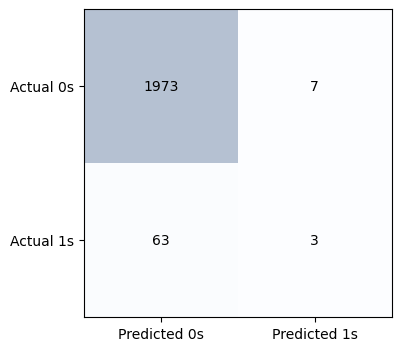
\includegraphics[width=6.5cm]{output_74_0.png}
    \caption{Matrica konfuzije za SVM metodu}
    \label{fig:galaxy}
\end{figure}

Primećujemo da da matrica konfuzije ima veliki broj grešaka prve vrste, što smo istakli kao veliku manu svakog modela.

Primenićemo sada SVM metodu na podatke koji su prethodno prošli SMOTE tehniku obrade, koristeći funkciju:


\hfill
\lstinputlisting[language=Python, firstline=242, lastline=243]
{kod.py}

\hfill

Posmatramo matricu konfuzije ovog modela i njenu grafičku reprezentaciju:

\begin{figure}[htp]
    \centering
    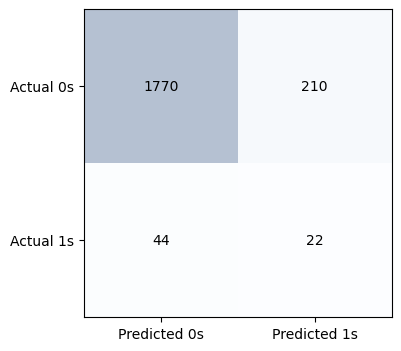
\includegraphics[width=6.5cm]{output_77_0.png}
    \caption{Matrica konfuzije za SVM metodu i SMOTE tehniku}
    \label{fig:galaxy}
\end{figure}
\newpage


Kao i do sad, kao mere kvaliteta u cilju procene performansi SVM modela u kombinaciji sa SMOTE tehnikom koristimo funkcije evaluacije  \emph{F1 Score}, \emph{AUC ROC} i \emph{Precision}. Njihovom primenom dobijamo sledeće rezultate:

\hfill
\lstinputlisting[language=Python, firstline=246, lastline=246]
{kod.py}
$$
\text{F1 Score : 0.54}
$$
$$
\text{AUC ROC : 0.61}
$$
$$
\text{Precision : 0.09}
$$

Primećujemo da su rezultati primetno bolji, tj. da se broj grešaka druge vrste povećao primenom SMOTE tehnike. Na osnovu vrednosti funkcija evaluacije zaključujemo da model ima određeni nivo efikasnosti, ali predikcije koje pravi ne mogu biti pouzdane.\\

Posmatrajmo sada primenu SVM metode na podacima na kojima su prethodno izvršeni PCA i SMOTE tehnika:

\hfill
\lstinputlisting[language=Python, firstline=248, lastline=249]
{kod.py}

\hfill

Posmatramo matricu konfuzije ovog modela i njenu grafičku reprezentaciju:

\begin{figure}[htp]
    \centering
    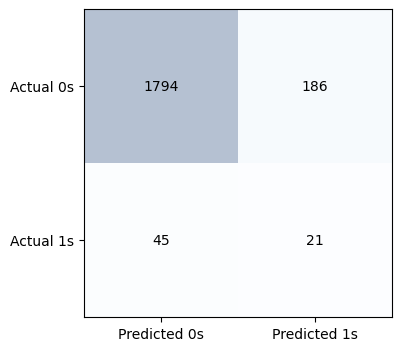
\includegraphics[width=7cm]{output_81_0.png}
    \caption{Matrica konfuzije za SVM metodu, PCA i SMOTE tehniku}
    \label{fig:galaxy}
\end{figure}

Kao i do sad, kao mere kvaliteta u cilju procene performansi SVM modela u kombinaciji sa PCA i SMOTE tehnikom koristimo funkcije evaluacije  \emph{F1 Score}, \emph{AUC ROC} i \emph{Precision}. Njihovom primenom dobijamo sledeće rezultate:

\hfill
\lstinputlisting[language=Python, firstline=252, lastline=252]
{kod.py}
$$
\text{F1 Score : 0.55}
$$
$$
\text{AUC ROC : 0.61}
$$
$$
\text{Precision : 0.10}
$$
\hfill

Na osnovu metrice konfuzije i već navedenih mera kvaliteta primećujemo da je razlika u kvalitetu modela zanemarljivo mala u odnosu na kvalitet SVM modela u kombinaciji sa SMOTE tehnikom. Ipak, obe metode daju bolje rezultate od metoda primenjenih na neuravnoteženim podacima.\\


Razmotrićemo kako izbor jezgra utiče na preciznost modela. Ponovićemo SVM metodu u kombinaciji sa SMOTE tehnikom, koristeći polinomijano jezgro na sledeći način:

\hfill
\lstinputlisting[language=Python, firstline=254, lastline=255]
{kod.py}

\hfill

Posmatramo matricu konfuzije ovog modela i njenu grafičku reprezentaciju:

\begin{figure}[htp]
    \centering
    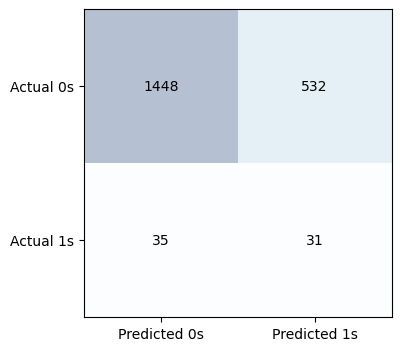
\includegraphics[width=7cm]{output_85_0.png}
    \caption{Matrica konfuzije za SVM metodu i SMOTE tehniku}
    \label{fig:galaxy}
\end{figure}

Kao i do sad, kao mere kvaliteta u cilju procene performansi SVM modela u kombinaciji SMOTE tehnikom koristimo funkcije evaluacije  \emph{F1 Score}, \emph{AUC ROC} i \emph{Precision}. Njihovom primenom dobijamo sledeće rezultate:

\hfill
\lstinputlisting[language=Python, firstline=258, lastline=258]
{kod.py}
$$
\text{F1 Score : 0.47}
$$
$$
\text{AUC ROC : 0.60}
$$
$$
\text{Precision : 0.06}
$$

\hfill

Matrica konfuzije SVM metode u kombinaciji sa SMOTE tehnikom korišćenjem polinomijalnog jezgra razlikuje se u odnosu matrice modela koji koriste drugačiji izbor jezgra. Međutim, vrednosti funkcije evaluacije ovog modela se skoro neprimetno razlikuju u odnosu na prethodne.\\

Posmatrajmo sada primenu SVM metode na podacima na kojima su prethodno izvršeni PCA i SMOTE tehnika:

\hfill
\lstinputlisting[language=Python, firstline=260, lastline=261]
{kod.py}

\hfill

Posmatramo matricu konfuzije ovog modela i njenu grafičku reprezentaciju:

\begin{figure}[htp]
    \centering
    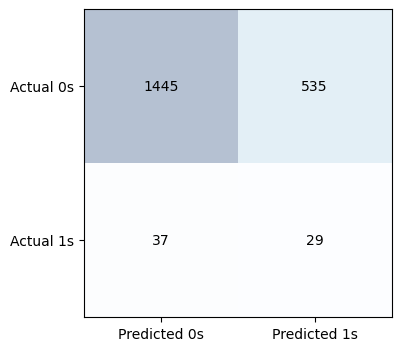
\includegraphics[width=7cm]{output_89_0.png}
    \caption{Matrica konfuzije za SVM sa polinomijalnim jezgrom}
    \label{fig:galaxy}
\end{figure}

Kao i do sad, kao mere kvaliteta u cilju procene performansi SVM modela u kombinaciji sa PCA i SMOTE tehnikom koristimo funkcije evaluacije  \emph{F1 Score}, \emph{AUC ROC} i \emph{Precision}. Njihovom primenom dobijamo sledeće rezultate:

\hfill
\lstinputlisting[language=Python, firstline=264, lastline=264]
{kod.py}
$$
\text{F1 Score : 0.46}
$$
$$
\text{AUC ROC : 0.58}
$$
$$
\text{Precision : 0.05}
$$

\hfill

Na osnovu metrice konfuzije i navedenih mera kvaliteta primećujemo da je razlika u kvalitetu modela nastalog upotrebom SVM metode u kombinaciji sa PCA i SMOTE tehnikom korišćenjem polinomijalnog jezgra mala u odnosu na modele koji koriste drugačiji izbor jezgra.


\subsection{XGBoost - Algoritam ektremnog gradijentnog pojačavanja}

Algoritam ekstremnog gradijentnog pojačavanja, tj. \emph{Extreme Gradient Boosting} je jedan od najefikasnijih i najpreciznijih algoritama za rešavanje problema klasifikacije i regresije.

Ovaj algoritam ima sposobnost da kombinuje veliki broj slabih modela, često predstavljenih u formi stabla odlučivanja, a zatim stvori jak i robustan model. Zasniva se na iterativnom procesu treniranja koji omogućava svakom stablu da se fokusira na greške prethodno izgrađenih stabala, čime se postepebo poboljšavaju performanse modela. 

Pored gorenavedenog, XGBoost algoritam ima ugrađenu podršku za paralelizaciju, što omogućava istovremeno izvršavanje računskih operacija na više procesora ili računarskih čvorova. Ova performansa smanjuje vreme potrebno za treniranje modela i poboljšava efikasnost prilikom obrade velikog broja podataka.

Takođe, algoritam daje informaciju o važnosti prediktora u modelu, te je lakše identifikotivati ključne faktore koji utiču na rezultate modela. XGBoost uključuje i različite tehnike regularizacije, te se lako prilagođava različitim problemima i skupovima podataka.

Primenićemo sada XGBoost algoritam na realne podatke iz naše baze na sledeći način:

\hfill
\lstinputlisting[language=Python, firstline=266, lastline=268]
{kod.py}

\hfill

Posmatramo matricu konfuzije ovog modela i njenu grafičku reprezentaciju:

\begin{figure}[htp]
    \centering
    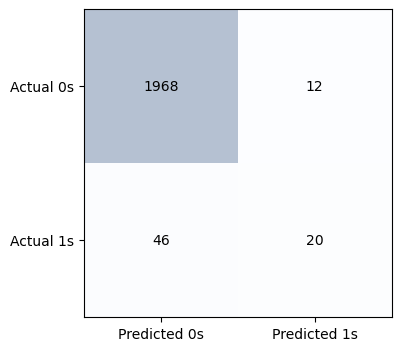
\includegraphics[width=7cm]{output_93_0.png}
    \caption{Matrica konfuzije za XGBoost metodu}
    \label{fig:galaxy}
\end{figure}

Donosimo iste zaključke kao prilikom analize SVM modela primenjenog na neuravnoteženim podacima.

Kao i do sad, kao mere kvaliteta u cilju procene performansi XGBOOST modela koristimo funkcije evaluacije  \emph{F1 Score}, \emph{AUC ROC} i \emph{Precision}. Njihovom primenom dobijamo sledeće rezultate:


\hfill
\lstinputlisting[language=Python, firstline=271, lastline=271]
{kod.py}
$$
\text{F1 Score : 0.70}
$$
$$
\text{AUC ROC : 0.65}
$$
$$
\text{Precision : 0.62}
$$
\hfill

Vidimo da su vrednosti funkcija evaluacije puno bolje u odnosu na prethodne. Ovo ukazuje da model nastao korišćenjem XGBoost metode ima primetno bolje performanse u odnosu na modele nastale korišćenjem ostalih metoda. \\

Razmotrimo sada implementaciju XGBoost metode na podacima na kojima je prethodno izvršena SMOTE tehnika:

\hfill
\lstinputlisting[language=Python, firstline=273, lastline=275]
{kod.py}

\hfill

Posmatramo matricu konfuzije ovog modela i njenu grafičku reprezentaciju:

\begin{figure}[htp]
    \centering
    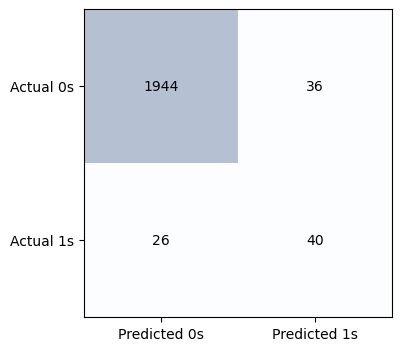
\includegraphics[width=7cm]{output_96_0.png}
    \caption{Matrica konfuzije za XGBoost metodu i SMOTE tehniku}
    \label{fig:galaxy}
\end{figure}

Kao i do sad, kao mere kvaliteta u cilju procene performansi SVM modela u kombinaciji sa PCA i SMOTE tehnikom koristimo funkcije evaluacije  \emph{F1 Score}, \emph{AUC ROC} i \emph{Precision}. Njihovom primenom dobijamo sledeće rezultate:

\hfill
\lstinputlisting[language=Python, firstline=278, lastline=278]
{kod.py}
$$
\text{F1 Score : 0.77}
$$
$$
\text{AUC ROC : 0.79}
$$
$$
\text{Precision : 0.53}
$$

\hfill

Vrednosti funkcija evaluacije ovog modela su malo bolje u odnosu na rezultate modela napravljenog na osnovu neuravnoteženih podataka. Ipak, preciznost predikcije modela napravljenom na podacima korišćenjem SMOTE tehnike je manja od preciznosti modela napravljenog na osnovu neuravnoteženih podataka.


\subsection{Random Forest - Algoritam slučajne šume}

Slučajna šuma, tj. \emph{Random Forest} je važan algoritam mašinskog učenja koji se takođe koristi za probleme klasifikacije i regresije.

Ovaj algoritam kombinuje više stabala odlučivanja u cilju postizanja boljeg rezultata. Naime, on generiše više stabala odlučivanja, pri čemu svako stablo radi sa nasumično izabranim podskupom podataka i prediktora. Valja napomenuti da je, zbog ovakvog načina implementacije, algoritam otporan na \emph{overfitting}, tj. preteranu prilagođenost modela. Kombinovanjem rezultata više stabala odlučivanja, Random forest uspeva da smanji disperziju i poveća stabilnost predikcija.

Random forest ima sposobnost rada sa podacima visoke dimenzije i velikim brojem prediktora. Kao i XGBoost, može proceniti važnost prediktora u okviru modela. Dakle, na osnovu odluka o razdvajanju podataka koje stabla donose, algoritam može izračunati važnost svakog prediktora i identifikovati one koji najviše doprinose predikciji.

Na nivou ansambla se može zadati broj stabala koja se treniraju ($\textit{n\_estimators}$ parametar), kao i svojstva koja prate stabla (kriterijum homogenosti, maksimalna dubina stabla, maksimalni broj atributa itd). Svojstvom $\textit{max\_depth}$ se može uticati na veličinu podskupa instanci nad kojim se stabla treniraju, dok je praksa da se kroz $\textit{random\_state}$ parametar prati slučajnost u podelama kako bi eksperimenti mogli da se reprodukuju.

Razmotrimo prvo kakve nam rezultate daje ovaj model kada su podaci neuravnoteženi.

\hfill
\lstinputlisting[language=Python, firstline=224, lastline=226]
{kod.py}

Posmatramo matricu konfuzije ovog modela i njenu grafičku reprezentaciju:

\begin{figure}[htp]
    \centering
    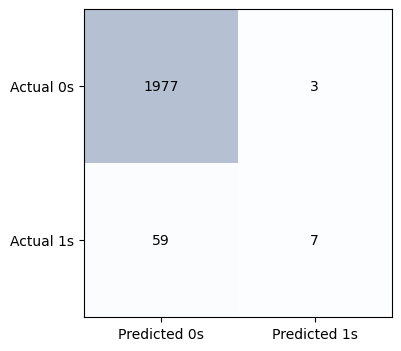
\includegraphics[width=7cm]{output_67_0.png}
    \caption{Matrica konfuzije za Random Forest metodu}
    \label{fig:galaxy}
\end{figure}

Ovi rezultati nisu zadovoljavajući jer je broj grešaka prve vrste znatno veći od broja grešaka druge vrste. U cilju poboljšanja našeg modela, pogledajmo šta će se desiti ako Random forest metod primenimo na podatke prethodne izbalansirane pomoću SMOTE tehnike.

\hfill
\lstinputlisting[language=Python, firstline=230, lastline=232]
{kod.py}

\hfill

Posmatramo matricu konfuzije ovog modela i njenu grafičku reprezentaciju:

\begin{figure}[htp]
    \centering
    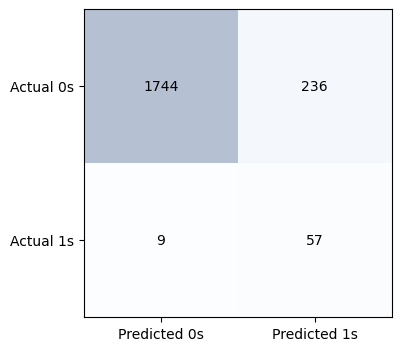
\includegraphics[width=7cm]{output_70_0.png}
    \caption{Matrica konfuzije za Random Forest metodu u kombinaciji sa SMOTE tehnikom}
    \label{fig:galaxy}
\end{figure}
\newpage
Vidimo da smo sada broj grešaka prvog tipa sveli na minimum i time značajno poboljšali preciznost našeg modela. Razmotrimo sada još i sledeće mere kvaliteta: funkcije evaluacije  \emph{F1 Score}, \emph{AUC ROC} i \emph{Precision}:

\hfill
\lstinputlisting[language=Python, firstline=235, lastline=235]
{kod.py}
$$
\text{F1 Score : 0.63}
$$
$$
\text{AUC ROC : 0.87}
$$
$$
\text{Precision : 0.19}
$$
\hfill

Vrednosti funkcije evaluacije dobijene ovim metodom su jako dobre, te možemo reći da nam je ovaj metod pružio dosad najveću preciznost i najmanju grešku prve vrste.

Random forest algoritam tokom treniranja modela, može proceniti važnost svakog atributa na osnovu toga koliko doprinosi smanjenju nečistoće ($\textit{impurity}$) ili gubitka informacija u modelu. Pošto su rezultati koje Random forest metod daje jako značajni, pogledajmo procenu važnosti atributa koju nam on daje. Na osnovu grafika možemo videti da za najvažnije atributie smatra $\textit{Net Value Per Share (C)}$ i $\textit{Gross Profit to Sales}$, dok neke atribute smatra potpuno nevažnim.


\begin{figure}[htp]
    \centering
    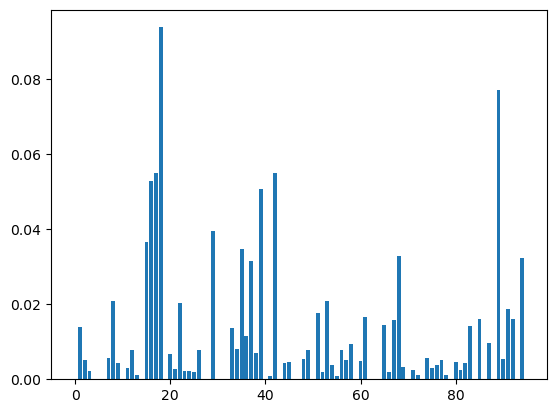
\includegraphics[width=7cm]{randomforestvaznost.png}
    \caption{Procena važnosti atributa za random forest model}
    \label{fig:galaxy}
\end{figure}


\newpage

\section{Zaključak}

\vspace{1cm}

U okviru ovog projekta imali smo prilike da pokažemo kako se mašinsko učenje i njegovi algoritmi mogu primeniti za predviđanje bankrota kompanije mnogo pre nego što se on desi.

Prilikom analize podataka upoznali smo se sa važnim konceptima mašinskog učenja poput redukcije dimenzionalnosti, izbora modela, evaluacije performansi i slično. U toku izrade projekta upoređivali smo rezultate dobijene različitim metodama, grafički ih prikazivali i donosili zaključke.

Na osnovu dobijenih rezultata možemo zaključiti da metode koje smo obradili imaju određeni uticaj na performanse modela predikcije bankrota. Međutim, primena većine metoda ne dovodi do značajnog poboljšanja u predikcijama. Kompleksnost obrane baze koja se sastoji od neuravnoteženih podataka i ostali faktori implicirali su malu pouzdanost modela predviđanja. 

Ipak, možemo konstatovati da smo najbolje modele dobili primenom Random forest modela na podatke izbalansirane korišćenjem SMOTE tehnike.

Važno je napomenuti da je baza koju smo koristili,kao i podaci koji su u njoj nalaze, usko vezana za prilike na tajvanskom berzi i da su tako dobijeni rezultati neprimenljivi za predviđanje bankrota kompanija u drugim državama. Da bismo uspešno predvideli poslovanje kompanije, bilo bi neophodno da skupimo dovoljno informacija o kompanijama iz iste države ili o kompanija koje posluju pod sličnim uslovima, te da nad tim podacima pravimo model koji će biti uspešan u prognoziranju.
\newpage

\begin{thebibliography}{9}
\vspace{1cm}
\bibitem{texbook}
Mladen Nikolić, Anđelka Zečević (2019).\emph{Mašinsko učenje}. Matematički fakultet., 1st ed.
\bibitem{textbook3}
Bojana Milošević (2019).\emph{Linearni statistički modeli}. Matematički fakultet., 1st ed.
\bibitem{textbook1}
Mihajlo Srbakoski (2023). Vežbe iz predmeta: \emph{Statistički softver 4}. Matematički fakultet.
\bibitem{textbook1} Saurabh Raj (2023).\emph{Company Bankruptcy Prediction}.

\bibitem{textbook1} Vishal Karmalkar, Shalin Shah,
Akshay Rajhans (2022).\emph{Bankruptcy Prediction on Real World Dataset using Machine Learning Algorithms}.

\bibitem{textbook1} Baza podataka korišćena za izradu projekta: \href{https://www.kaggle.com/datasets/fedesoriano/company-bankruptcy-prediction?resource=download}{\emph{Company Bankruptcy Prediction}}.


\end{thebibliography}.

\end{document}
